\documentclass[10pt,a5paper]{extarticle}
\usepackage[margin=.7cm]{geometry}
\usepackage[utf8]{inputenc}
\usepackage[IL2]{fontenc}
\usepackage[czech]{babel}
\usepackage{microtype}
\usepackage{amssymb}
\usepackage{amsthm}
\usepackage{amsmath}
\usepackage{xcolor}
\usepackage{graphicx}
\usepackage{wasysym}

\usepackage[inline]{enumitem}

\newcommand{\R}{\mathbb{R}}

\newcommand{\hint}[1]{{\color{gray}\footnotesize\noindent(Nápověda: #1)}}

\DeclareMathOperator{\tg}{tg}
\DeclareMathOperator{\cotg}{cotg}

\setlist[enumerate]{label={(\alph*)},topsep=\smallskipamount,itemsep=\smallskipamount,parsep=0pt,itemjoin={\quad}}
\setlist[itemize]{topsep=\smallskipamount,noitemsep}

\def\tisk{%
\newbox\shipouthackbox
\pdfpagewidth=2\pdfpagewidth
\let\oldshipout=\shipout
\def\shipout{\afterassignment\zdvojtmp \setbox\shipouthackbox=}%
\def\zdvojtmp{\aftergroup\zdvoj}%
\def\zdvoj{%
    \oldshipout\vbox{\hbox{%
        \copy\shipouthackbox
        \hskip\dimexpr .5\pdfpagewidth-\wd\shipouthackbox\relax
        \box\shipouthackbox
    }}%
}}%

\let\results\newpage
\let\endresults\relax

\def\resultssame{%
    \long\def\results##1\endresults{%
        \vfill\noindent\rotatebox{180}{\vbox{##1}}%
    }%
}


\newtheorem*{poz}{Pozorování}

\theoremstyle{definition}
\newtheorem{uloha}{\atr Úloha}
\newtheorem{suloha}[uloha]{\llap{$\star$ }Úloha}
\newtheorem*{bonus}{Bonus}
\newtheorem*{defn}{Definice}

\pagestyle{empty}

\let\ee\expandafter

\def\vysld{}
\let\printvysl\relax
\let\printalphvysl\relax

\makeatletter
\long\def\vyslplain#1{\ee\ee\ee\gdef\ee\ee\ee\vysld\ee\ee\ee{\ee\vysld\ee\printvysl\ee{\the\c@uloha}{#1}}}
\let\vysl\vyslplain

\def\locvysl#1{\ee\gdef\ee\locvysld\ee{\locvysld\item #1}}
\let\lv\locvysl

\newenvironment{ulohav}[1][]{\begin{uloha}[#1]\gdef\locvysld{\begin{enumerate*}}}{\ee\vyslplain\ee{\locvysld\end{enumerate*}}\end{uloha}}
\def\stitem{\@noitemargtrue\@item[$\star$ \@itemlabel]}

\makeatother

\def\atr{}
\def\basic{\def\atr{\llap{\mdseries$\sun$ }\gdef\atr{}}}
\def\interest{\def\atr{\llap{$\star$ }\gdef\atr{}}}
\def\iinterest{\def\atr{\llap{$\star\star$ }\gdef\atr{}}}
\let\mb\mathbf


\begin{document}
% Toto je z mého pohledu hrozně krásná sada úloh, ale v reálu je její použitelnost
% diskutabilní. Zřejmě není možné ji "jen tak" rozdat studentům bez dalšího komentáře.

%\tisk
%\resultssame

\section*{Geometrické důkazy}


\begin{uloha}
Dokažte vzorec pro obsah trojúhelníka $S = \frac12 a v_a$ ($v_a$ = výška na stranu $a$). \hint{\uv{Doplňte} trojúhelník na obdélník.} Zvládnete to i pro \emph{tupoúhlý}?
\[ 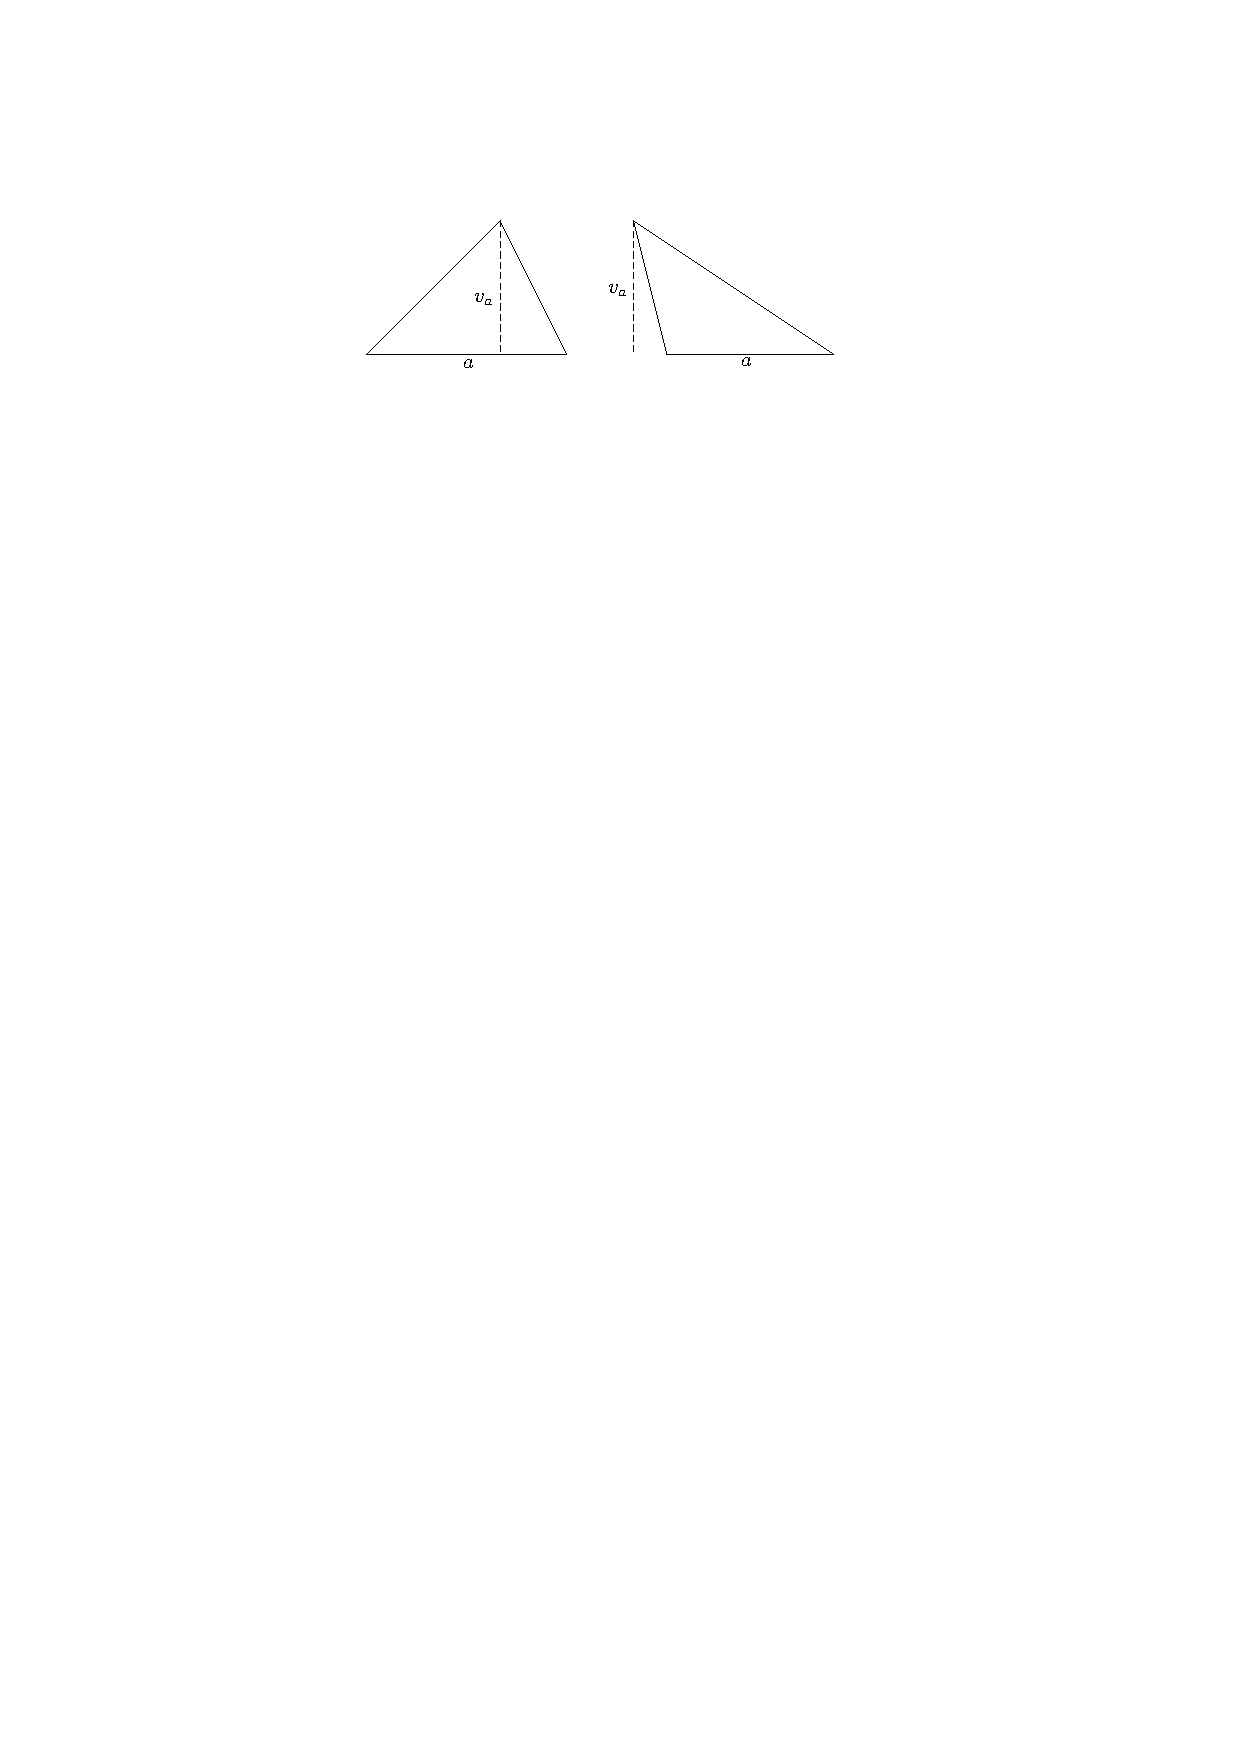
\includegraphics{trojuh_obsah.pdf} \]
\end{uloha}


\begin{uloha}
Uvažme pravoúhlý trojúhelník rozdělený výškou z vrcholu $C$ (naproti přeponě); označíme $D$ patu oné výšky a $c_a = |BD|$, $c_b = |AD|$.
\[ 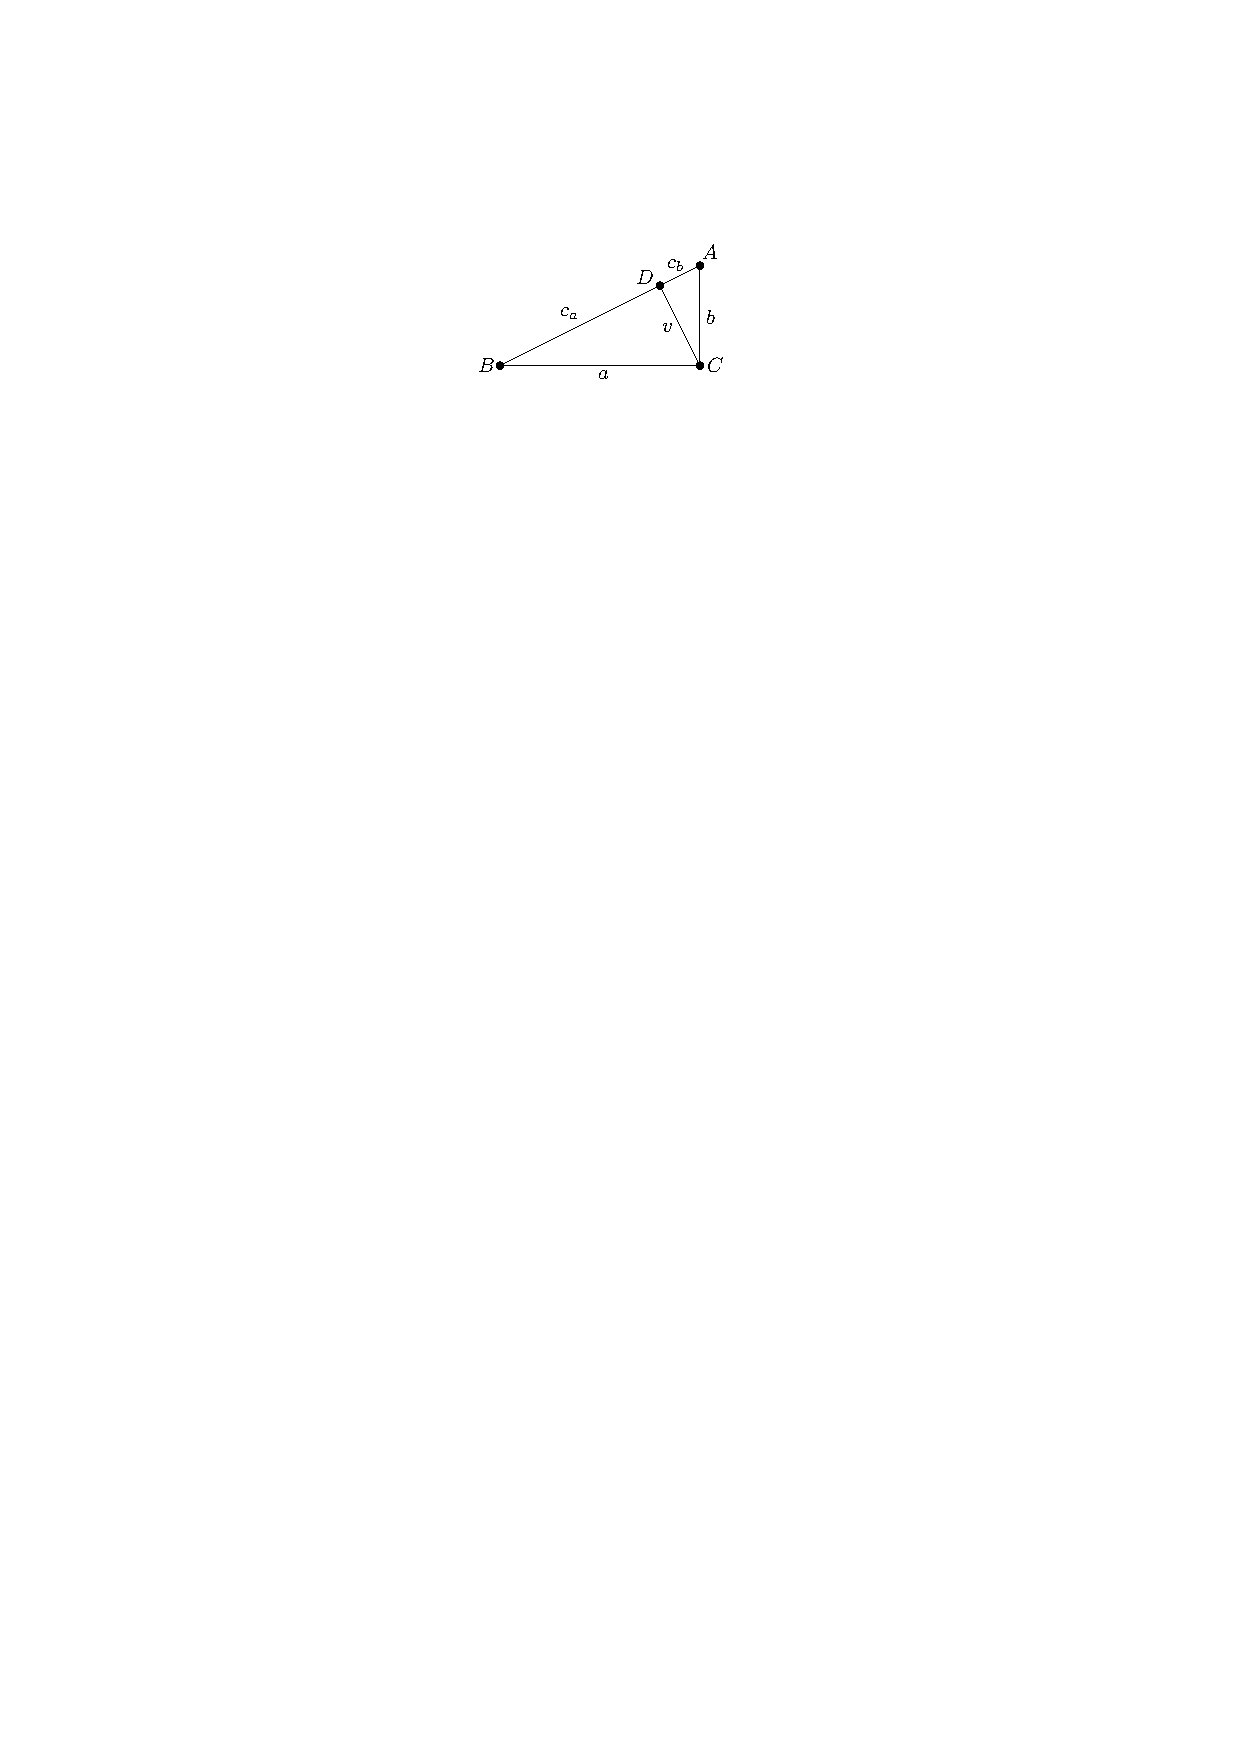
\includegraphics{pravouh.pdf} \]
\begin{enumerate}
    \item Zdůvodněte, proč jsou všechny tři trojúhelníky na obrázku podobné; které vrcholy si odpovídají? \hint{Stačí porovnat vnitřní úhly.}
    \item Doplňte poměry podle podobností z předchozího bodu: $a:b:c = \boxed{\phantom{i}}:\boxed{\phantom{i}}:\boxed{\phantom{i}} = \boxed{\phantom{i}}:\boxed{\phantom{i}}:\boxed{\phantom{i}}$.
    \item Dokažte \emph{Euklidovu větu o výšce}: $v = \sqrt{c_a \cdot c_b}$. \hint{Stačí zkombinovat příslušné dva poměry z předchozího bodu.}
    \item Dokažte \emph{Euklidovu větu o odvěsně}: $a = \sqrt{c \cdot c_a}$, $b = \sqrt{c \cdot c_b}$.
    \item Dokažte \emph{Pythagorovu větu}: $a^2 + b^2 = c^2$. \hint{Dosaďte z Euklidovy věty o odvěsně.}
\end{enumerate}
\end{uloha}

\begin{uloha}
Dokažte \emph{Thaletovu větu}: Je-li úsečka $AB$ průměrem kružnice $k$ a $C$ libovolný bod $k$ různý od $A$, $B$, pak je úhel $ACB$ pravý.
\[ 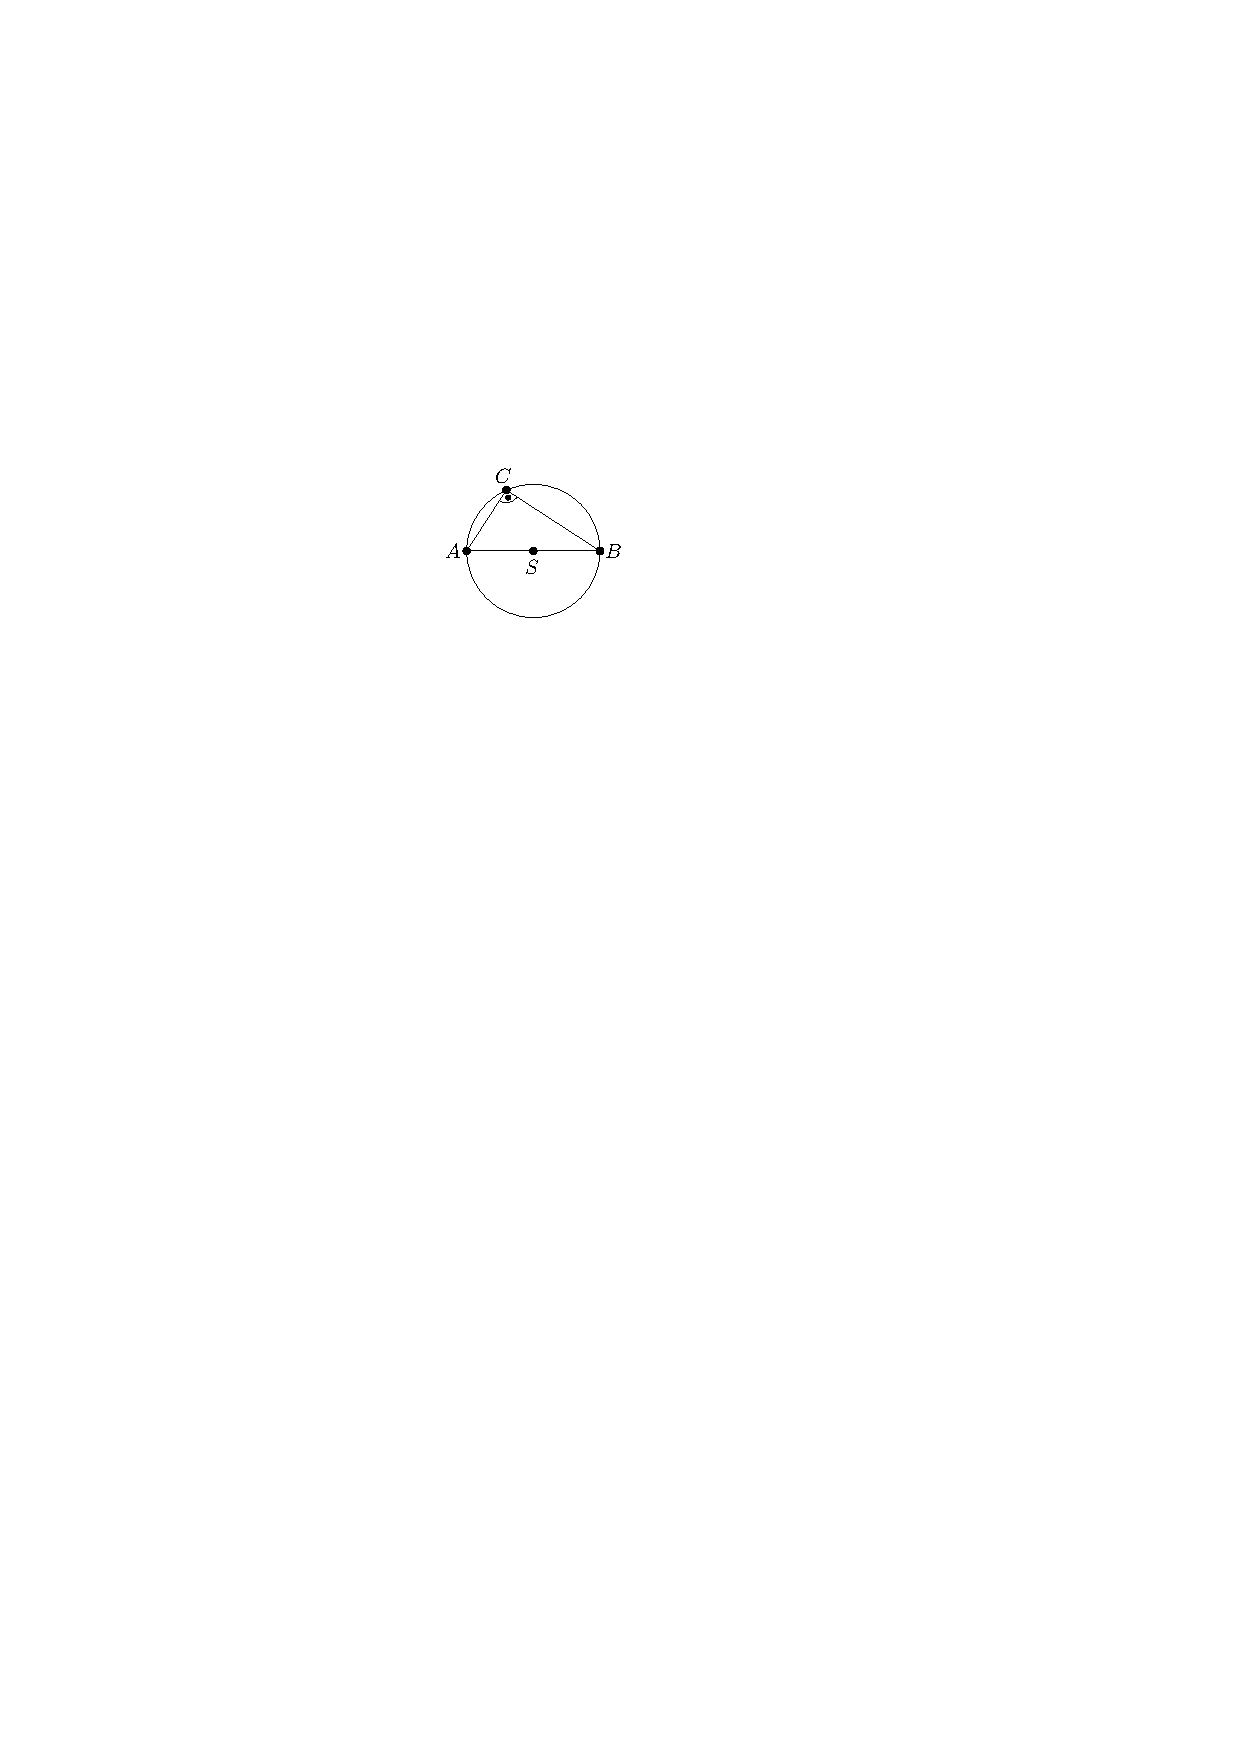
\includegraphics{thales.pdf} \]
\hint{Doplňte si do obrázku úsečku $CS$ a počítejte úhly. Jsou tam rovnoramenné trojúhelníky.}
\end{uloha}

\interest
\begin{uloha}
Dokažte \emph{Větu o středovém a obvodovém úhlu}: Máme-li kružnici se středem $S$, tři různé body $A$, $B$, $C$ na jejím obvodu takové, že $S$ leží uvnitř úhlu $ACB$,\footnote{Tvrzení platí do jisté míry i bez této podmínky.} tak platí $|\sphericalangle ASB| = 2 \cdot |\sphericalangle ACB|$. \hint{Doplňte úsečky a dopočtěte úhly; opět rovnoramenné trojúhelníky.}
\end{uloha}


\interest
\begin{uloha}
\emph{Tětivový čtyřúhelník} je takový, kterému lze opsat kružnice.
\[ 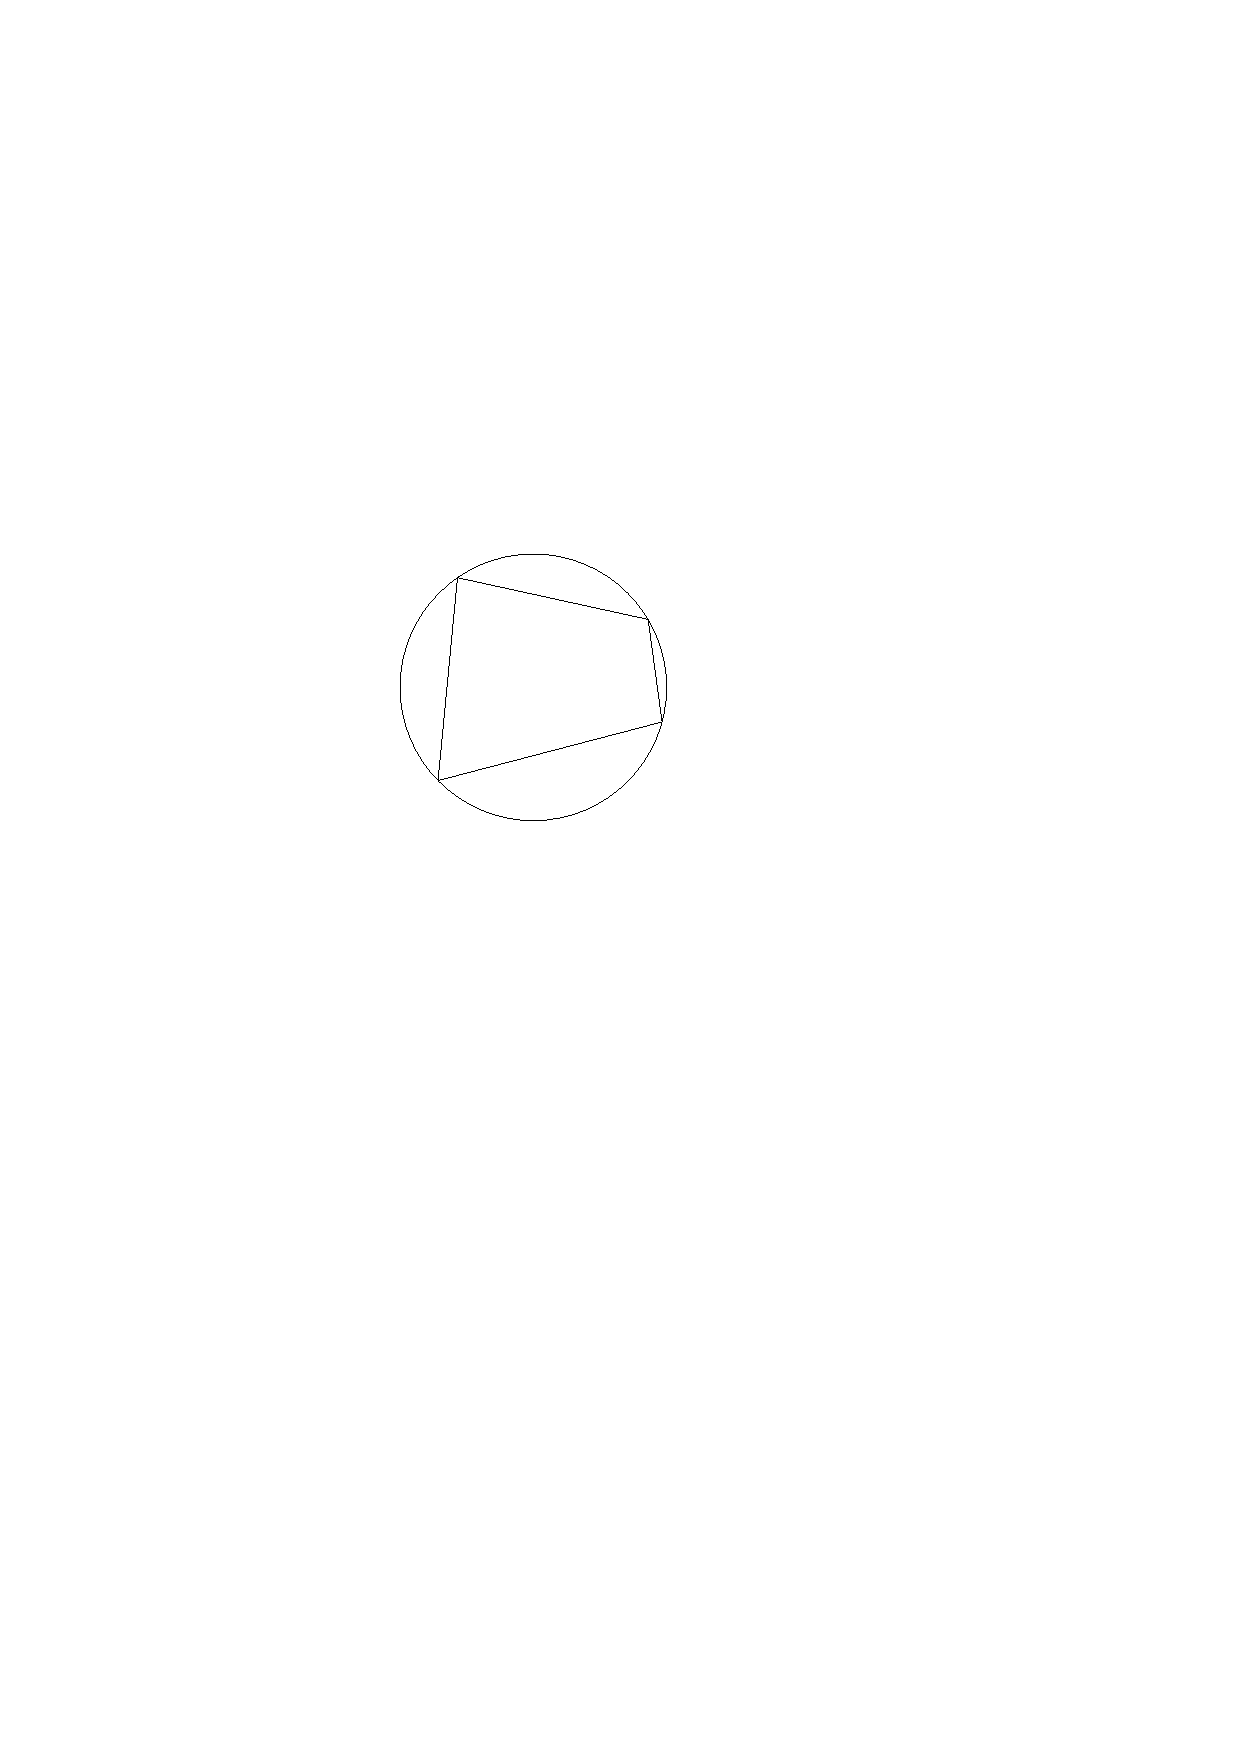
\includegraphics{tetivak.pdf} \]
Dokažte, že součet protějších úhlů v každém tětivovém čtyřúhelníku je $180^\circ$.
\hint{Doplňte si do obrázku spojnice vrcholů se středem a počítejte úhly. Jsou tam rovnoramenné trojúhelníky.}
\end{uloha}


\end{document}